\section{Modeling Metabolites using UKF}
\label{Modeling Metabolites using UKF}




\noindent This is the same system explored in chapter 3.2, but explored in the context of using an UKF as opposed to an EKF. The original research used an adaptation of the UKF, called the Iterative Unscented Kalman Filter (IUKF), to model the biological pathway of metabolites. Recall that this model contains four different states and 18 unknown parameters. These researchers utilized the IUKF for parameter fitting and was useful in enabling the model converge faster by resetting the covariance to re-excite the model. By not resetting the covariance at this step (as is done in the UKF), the three state variables without measurements converge significantly slower in this model. Utilizing the IUKF on this model was effective, because data regarding metabolites is highly influenced by noise, which is a factor that makes other approaches, such as regression and annealing, fail \cite{article5}. \\ 

\noindent  \\ 

\noindent In the paper, researchers had access to their own data sources and used an approach that was adapted from the UKF. Though we are not using their exact dataset, we will be simulating data using the same approach as the previous example. However, this example will be following UKF algorithm, as opposed to the IUKF algorithm. By doing so, the state variables without incoming measurements converge significantly slower than the measurable states. Ultimately, the goal of this example is to demonstrate how the UKF works on higher dimensional and more complex systems. \\
%how the UKF can correct for multiple variables or states, and how parameters can be adjusted to fit the model. \\ 

\noindent Recall that the four metabolites have the following differential equations:
\begin{align*}
\dot x_1 &= \alpha_1 x_3^{g_{13}} x_5^{g_{15}} - \beta_1 x_1^{h_{11}}, \\
\dot x_2 &= \alpha_2 x_1^{g_{21}} - \beta_2 x_2^{h_{22}}, \\
\dot x_3 &= \alpha_3 x_2^{g_{32}} - \beta_3 x_3^{h_{33}} x_4^{h_{34}}, \\
\dot x_4 &= \alpha_4  x_1^{g_{41}} - \beta_4 x_4^{h_{44}},
\end{align*}
with 18 parameters ($\alpha_1, \hdots, \alpha_4, \beta_1, \hdots, \beta_4, g_{13}, g_{15}, g_{21}, \\ g_{32}, g_{41}, h_{11}, h_{22}, h_{33}, h_{34}, h_{44} $). Unlike in chapter 3.2, we are not estimating parameters, so this system will use the true parameters in every time step. In both the original example as well as this one, sampling time will be 0.1 seconds for 5 seconds, totaling 50 UKF estimates. Recall that data is simulated on MATLAB and the model is initialized with state variable $x_0 = [4, 1, 3, 4]^T$ and the state covariance to $P_0 = .01I$. 


\begin{figure}[h]
    \centering
    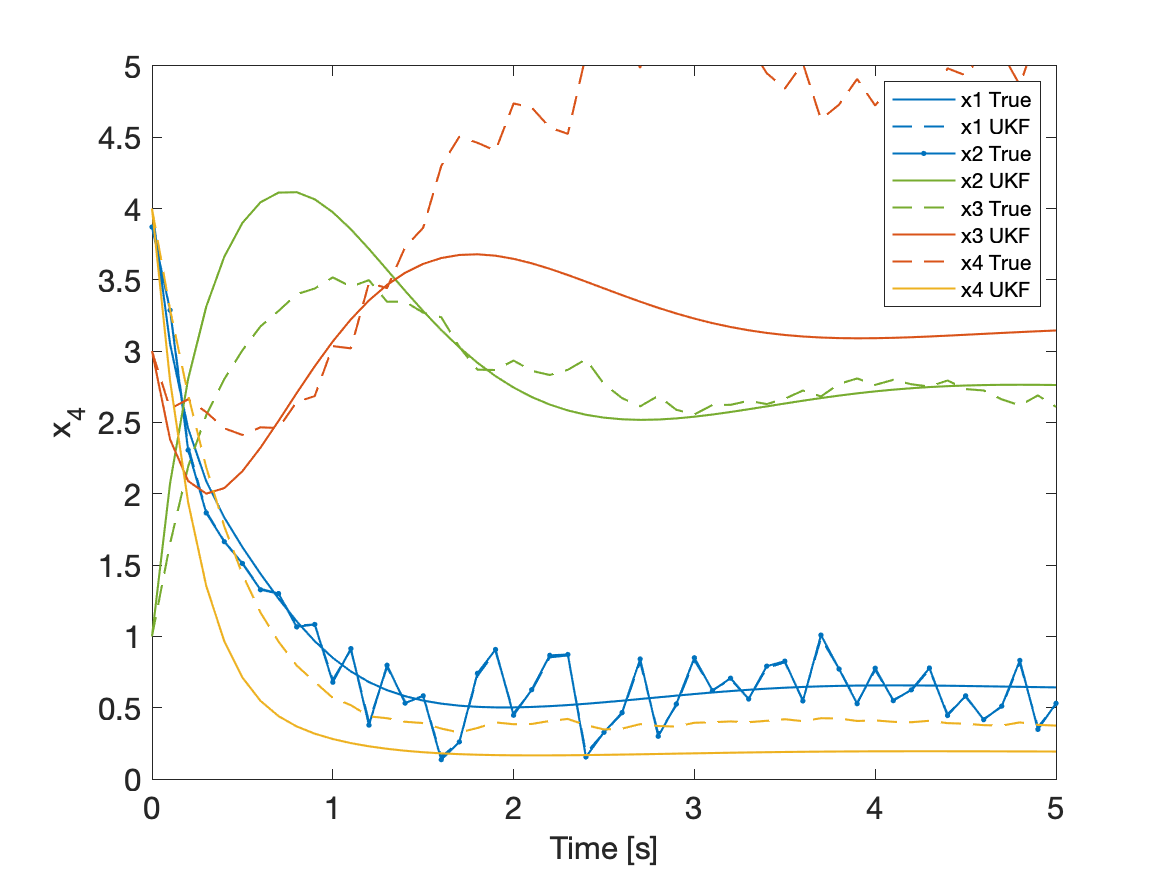
\includegraphics[scale = 0.6]{Meskin_overall.png}
    \caption{Performance of all state variables with the following conditions: R = 0.001, Q = (0.02 0.01 .03 .04) and initial values = $[4, 1, 3, 4]^T$.}
    %Paramaters included:  }% $, \alpha = 1, \kappa = 0  }
\end{figure}

\noindent Since the first state, $x1$ is the only state that has incoming system measurements, we have a 3 different blue lines in this figure. From this figure, it appears that the UKF prediction perfectly overlaps with the measured values. However, upon closer inspection, it actually does not. This is likely because there is only a small amount of measurement noise to the system. Figure 4.9 highlights the same information as Figure 4.8, but separates the states into different graphs, enabling a clearer illustration of each state's behavior.

\begin{figure}[h]
    \centering
    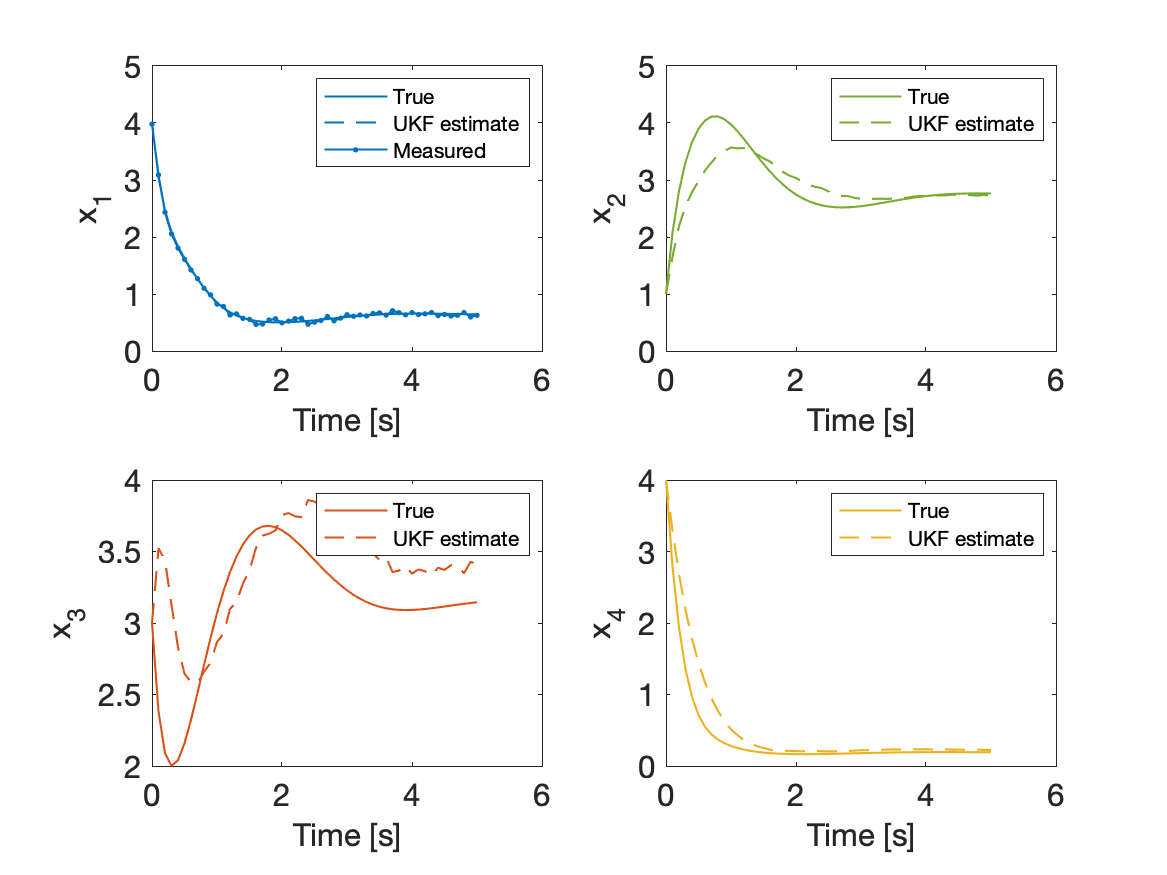
\includegraphics[scale = 0.6]{Meskin_states.png}
    \caption{Performance of all four state variables with one corrected state. The first state variable (blue) is the only one that is receiving measurements from the system. This explains why it is more accurate and converges better with the system, as compared with the other three states.}
    \label{map}
\end{figure}

\noindent In the original example, researchers used the following parameter values: $\epsilon = 1, \kappa = -14$. In theory, values of $\kappa$ can be negative, but negative values cannot be inputted into MATLAB. Therefore, the parameter values used in this example are set to default values ($\alpha = 1e-3, \beta = 2, \kappa = 0$). \textcolor{red}{Expand here on tweaking parameters}.\\

\noindent Residuals, also known as the innovation, are one way to access the model's performance. Recall that the residual is the difference between the actual measurement values and the predicted measurement values. Since only one state, $x1$ had incoming measurements, the residual graph in Figure 4.10 is specifically for $x1$. Generally, a strong residual graph has
\begin{itemize}
\item a symmetrical distribution that is clustered toward the center,
\item values that are close to 0,
\item a random or unclear pattern.
\end{itemize}
Figure 4.10 exhibits these three characteristics, indicating strong model performance. 

\begin{figure}[h]
    \centering
    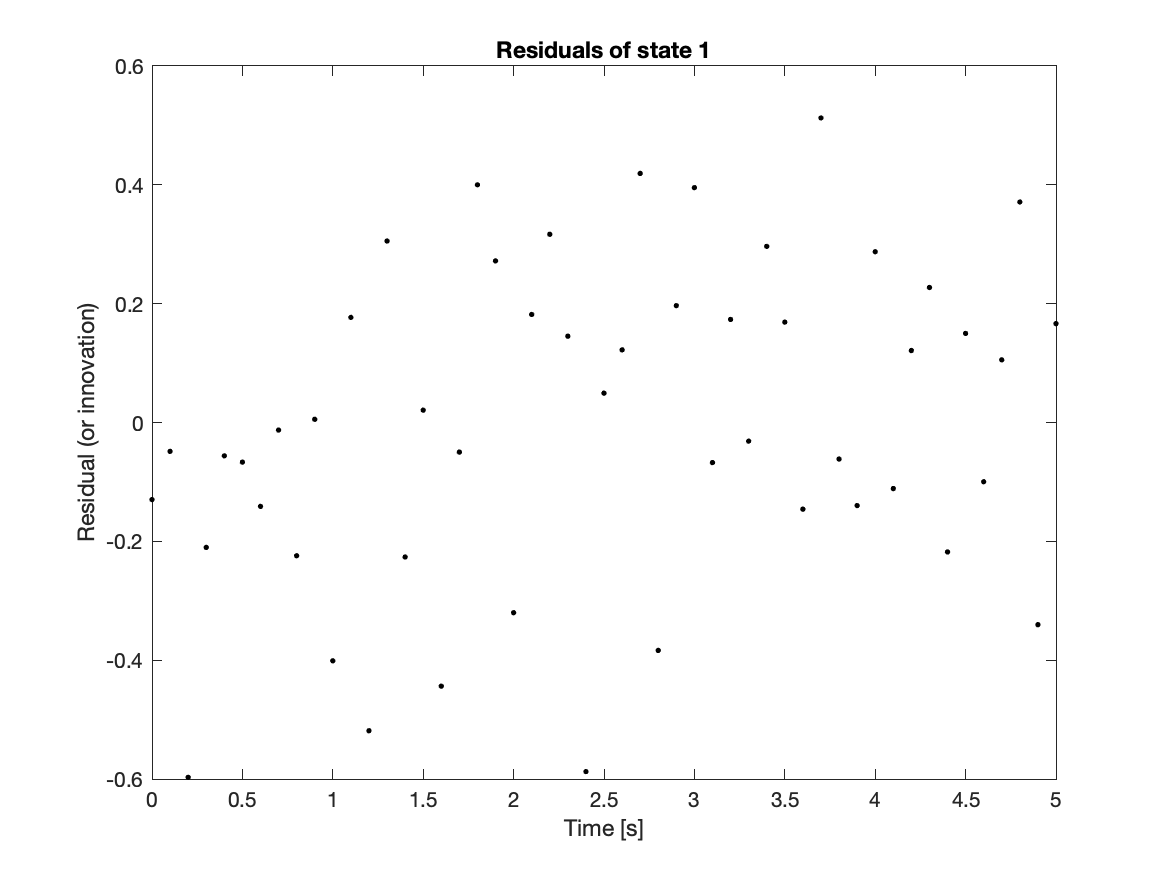
\includegraphics[scale = 0.6]{Meskin_residuals_state1.png}
    \caption{This scatterplot provides information regarding the residual, or innovation, of the first state, which is the only state recieving incoming system measurements.}
\end{figure}


\noindent Future work includes using the UKF for parameter fitting. One approach would be to use a technique similar to the one employed in chapter 3.2. Alternatively, another non-linear Kalman Filter technique, known as the Dual Unscented Kalman Filter, may also be a promising solution. Either of these two methods will likely be better than the method used in chapter 3.2, because calculating the exponential matrix and jacobian of the system is very computationally expensive and can be avoided with the UKF.

%\noindent \textcolor{red}{Expand here on correcting for 1+ states, currently we are having technical challenges in completing this step}













